\documentclass[10pt]{beamer}
\usetheme{jambro}

\title[]{Pensamento Econômico Contemporâneo - Modelo clássico}
\author[]{Paulo Victor da Fonseca}
\date{}

\hypersetup{
    colorlinks = true,
    urlcolor = teal,
    linkcolor = teal    
}
\usepackage[portuguese]{babel}
\usepackage{subfig}
\usepackage{emoji}

\begin{document}

\begin{frame}[plain]
    \titlepage{
        \begin{center}
            \begin{minipage}{0.8\textwidth}
                \centering
            \end{minipage}
        \end{center}}
\end{frame}

\begin{frame}{Sumário}
    \tableofcontents
\end{frame}

\section{Introdução}
\begin{frame}{Introdução}
    \begin{itemize}
        \item Para compreender as teorias macro atuais é necessário retomar suas origens ao debate Keynes vs. clássicos da década de 1930 que permanece, de formas distintas, até hoje\bigskip

        \item 1980s: as duas escolas no centro do debate macro eram representadas pelas teorias novo-clássicas e de RBC e a escola novo-Keynesiana\bigskip

        \item RBC - tradição clássica ao enfatizar a força otimizadora de agentes econômicos em um ambiente das forças do livre mercado\bigskip

        \item NK - flutuações econômicas requerem não apenas as complexidades do equilíbrio geral mas, também, admitem possibilidade de falhas de mercado em larga escala
    \end{itemize}
\end{frame}

\begin{frame}{Introdução}
    \begin{itemize}
        \item \tikz[tstyle]{\node[nstyle](node0){Economia clássica}}: corpo teórico existente no período anterior à publicação da Teoria Geral\bigskip
              \begin{tikzpicture}[tpstyle]
                  \node[pencil,draw,minimum height=0.5cm,minimum width=3cm] (box0) at (node0) {};
              \end{tikzpicture}

        \item Keynes: escola clássica incluía não apenas Smith, Ricardo e Mill. Mas, também, trabalhos de seguidores de Ricardo que adotaram e aperfeiçoaram a teoria Ricardiana\bigskip

        \item Classificação distinta da ortodoxia de HPE, especialmente pela inclusão de Marshall e Pigou como clássicos
    \end{itemize}
\end{frame}

\begin{frame}
    {Introdução}    
        \begin{figure}
            \centering
            \subfloat[\href{https://pt.wikipedia.org/wiki/Adam_Smith}{Adam Smith}\label{fig1a}]{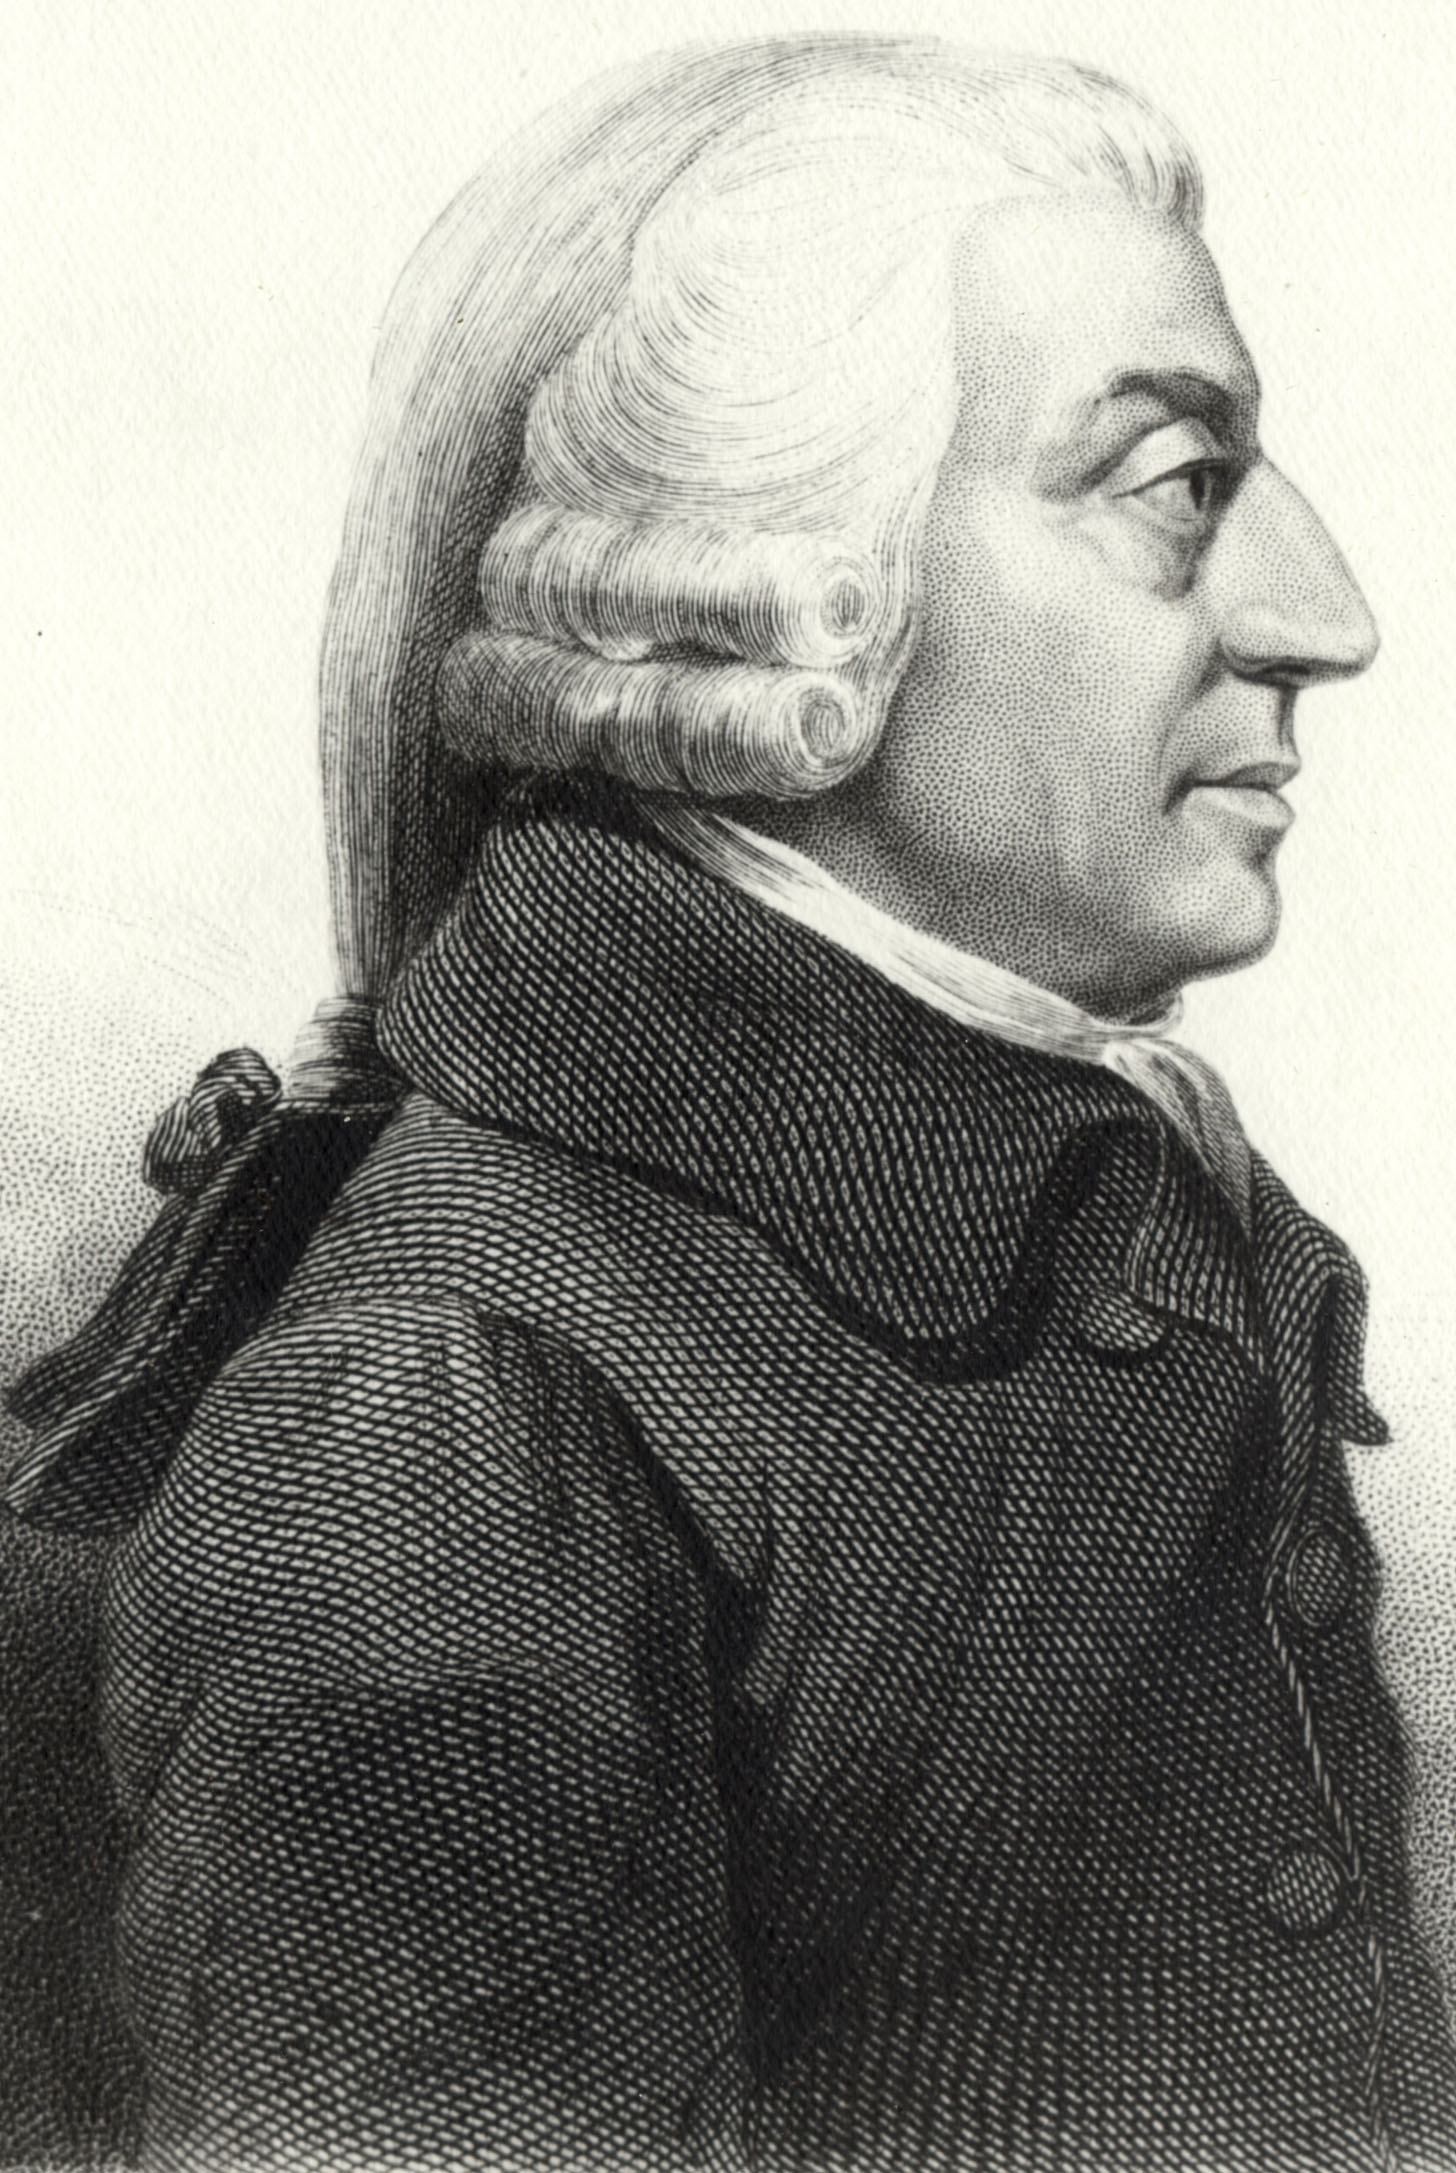
\includegraphics[width=0.25\textwidth]{./figures/aula2_smith.jpg}} \qquad
            \subfloat[\href{https://pt.wikipedia.org/wiki/David_Ricardo}{David Ricardo}\label{fig1b}]{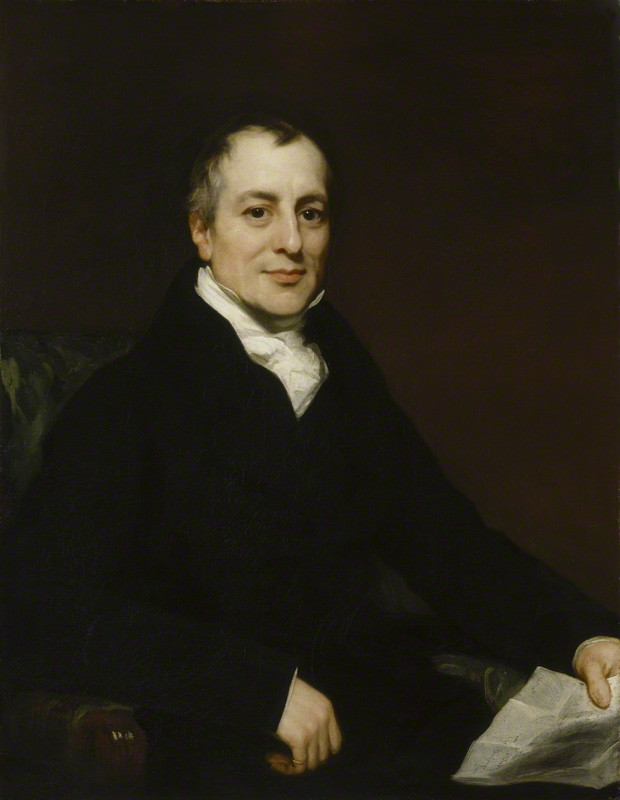
\includegraphics[width=0.25\textwidth]{./figures/aula02_ricardo.jpg}} \qquad
            \subfloat[\href{https://pt.wikipedia.org/wiki/John_Stuart_Mill}{John Stuart Mill}\label{fig1c}]{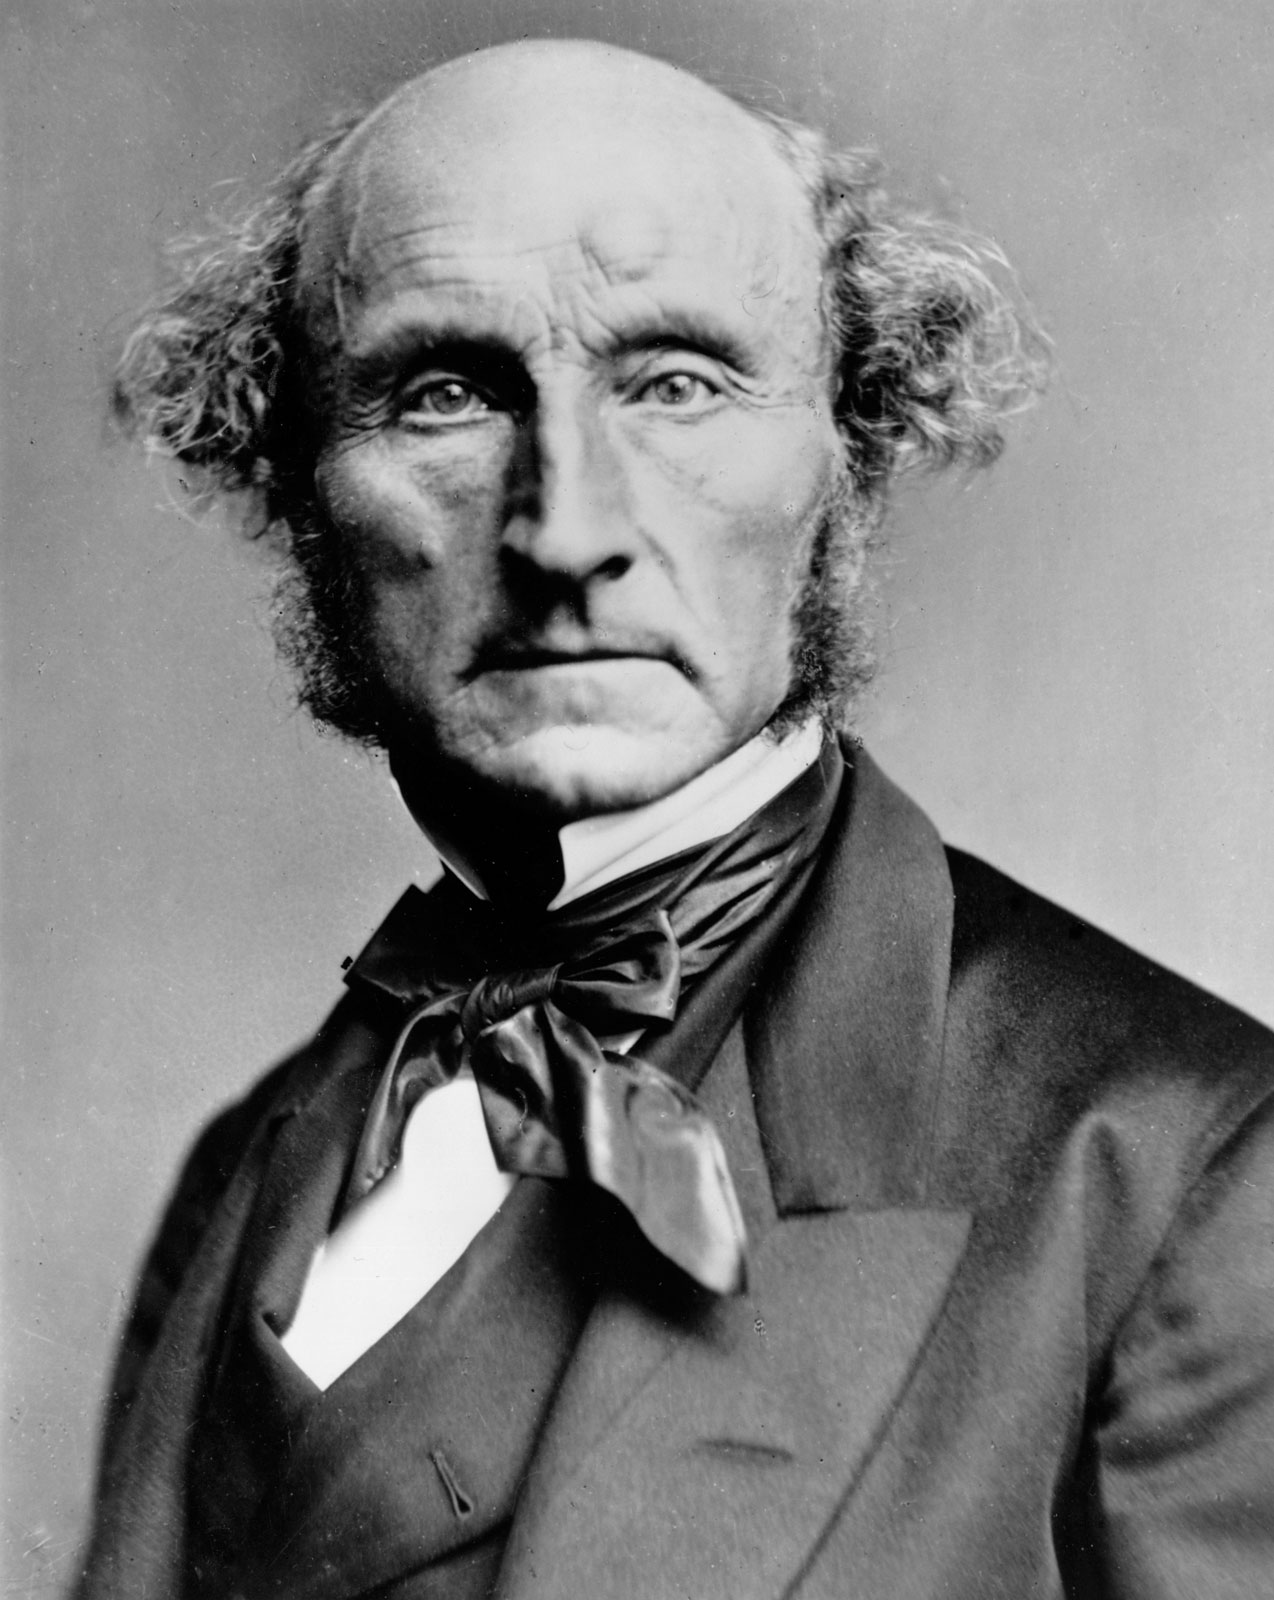
\includegraphics[width=0.25\textwidth]{./figures/aula02_mill.jpg}}
            \caption{Economistas clássicos}
            \label{fig1}
        \end{figure}    
\end{frame}

\begin{frame}
    {Introdução}    
        \begin{figure}
            \centering
            \subfloat[\href{https://pt.wikipedia.org/wiki/Alfred_Marshall}{Alfred Marshall}\label{fig2a}]{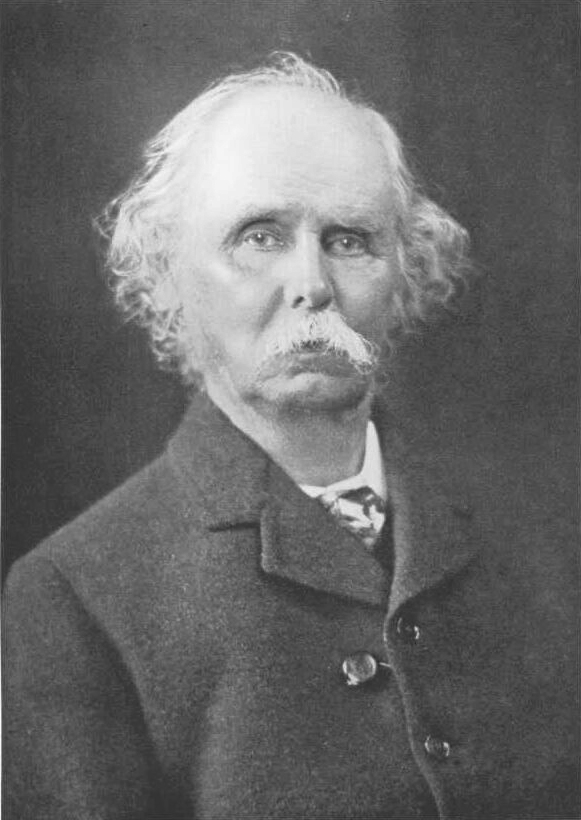
\includegraphics[width=0.25\textwidth]{./figures/aula02_marshall.jpg}} \qquad
            \subfloat[\href{https://pt.wikipedia.org/wiki/Arthur_Cecil_Pigou}{Arthur Cecil Pigou}\label{fig2b}]{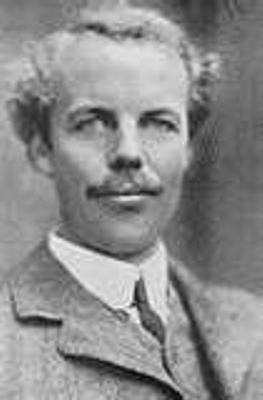
\includegraphics[width=0.25\textwidth]{./figures/aula02_pigou.jpg}}
            \caption{Economistas clássicos}
            \label{fig2}
        \end{figure}    
\end{frame}

\begin{frame}{Introdução}
    \begin{itemize}
        \item A maior parte dos avanços teóricos que distinguem a economia clássica da neoclássica deu-se na teoria micro\bigskip

        \item Keynes, por sua vez, argumenta que as ideias macro do período 1776-1936 eram razoavelmente homogêneas em termos de `mensagens gerais': crença nos mecanismos naturais de ajustamento de mercados em assegurar e manter um equilíbrio de pleno emprego\bigskip

        \item Cabe ressaltar, no entanto, que antes da Teoria Geral, não existia uma teoria unificada e formalizada do emprego agregado, e diferenças substanciais existiam acerca da natureza e origem dos ciclos de negócios
    \end{itemize}
\end{frame}

\begin{frame}{Introdução}
    \begin{itemize}
        \item A estrutura da macro clássica emergiu, de maneira geral, após 1936 e, em grande parte, em resposta à obra de Keynes até para que comparações fossem possíveis\bigskip

        \item Aqui adotaremos uma abordagem convencional ao apresentar um resumo artificial da macro clássica, um campo de pesquisa que, na realidade, era complexa e diversa\bigskip

        \item No entanto, essa abordagem é extremamente útil para que possamos compreender, mesmo que de forma simplificada, tanto as posições clássicas quanto keynesianas
    \end{itemize}
\end{frame}

\section{Macroeconomia clássica}
\begin{frame}{Macroeconomia clássica}
    \begin{itemize}
        \item Economistas clássicos sabiam que uma economia capitalista de mercado poderia apresentar desvios com relação ao emprego e produto de equilíbrio\bigskip

        \item No entanto, tais distúrbios seriam temporários e breves: os mecanismos de mercado operariam de maneira  rápida e eficiente para restaurar o equilíbrio de pleno emprego\bigskip

        \item Intervenções governamentais (na forma de políticas ativistas de estabilização) não seriam nem necessárias ou desejáveis\bigskip

        \item Na verdade, segundo esta visão, é mais provável que tais políticas causem ainda mais instabilidades
    \end{itemize}
\end{frame}

\begin{frame}{Macroeconomia clássica}
    \begin{itemize}
        \item Visão compartilhada por teóricos modernos seguidores da tradição clássica. A teoria novo-clássica RBC compartilha essa crença na força otimizadora dos mecanismos de mercado e do potencial das intervenções ativistas governamentais em criar mais danos que benefícios\bigskip

        \item Segue, portanto, que \hlight{economistas cl\'{a}ssicos davam pouca aten\c{c}\~{a}o tanto aos fatores determinantes da demanda agregada quanto \`{a}s pol\'{i}ticas de estabiliza\c{c}\~{a}o da demanda agregada que buscam assegurar o pleno emprego}\bigskip

        \item Para economistas clássicos, o pleno emprego era o estado natural do sistema econômico\bigskip

        \item Que Keynes atacaria estas ideias nos anos 1930s não é surpresa: desemprego em massa nas economias capitalistas - Grande Depressão
    \end{itemize}
\end{frame}

\subsection{Características do modelo}
\begin{frame}{Pressupostos do modelo clássico}
    \begin{itemize}
        \item Nas próximas aulas apresentaremos uma versão estilizada do modelo clássico que objetiva explicar os determinantes do nível de produto real ($Y$), salários reais ($W/P$) e nominais ($W$), nível de preços ($P$) e taxa real de juros ($r$)\bigskip

        \item Pressupostos assumidos pelo modelo:\medskip
              \begin{enumerate}
                  \item \tikz[tstyle]{\node[nstyle](node2){Agentes econômicos racionais e maximizadores de lucros ou utilidade}}; além disso, não sofrem ilusão monetária\medskip
                        \begin{tikzpicture}[tpstyle]
                            \draw[pencil, thick] ([yshift=-1pt]node2.south west) to ([yshift=-1pt]node2.south east);
                        \end{tikzpicture}

                  \item \tikz[tstyle]{\node[nstyle](node2){Mercados perfeitamente competitivos}} - agentes são tomadores de preços, que são completamente flexíveis\medskip
                        \begin{tikzpicture}[tpstyle]
                            \draw[pencil, thick] ([yshift=-1pt]node2.south west) to ([yshift=-1pt]node2.south east);
                        \end{tikzpicture}
                  \item \tikz[tstyle]{\node[nstyle](node2){Todos os agentes possuem informações perfeitas acerca das condições de mercado e preços}}\medskip
                        \begin{tikzpicture}[tpstyle]
                            \draw[pencil, thick] ([yshift=-1pt]node2.south west) to ([yshift=-1pt]node2.south east);
                        \end{tikzpicture}
                  \item \tikz[tstyle]{\node[nstyle](node2){Transações efetivadas após estabelecidos os preços de equilíbrio em todos os mercados}} - assegurado pela figura de um leiloeiro Walrasiano fictício\medskip
                        \begin{tikzpicture}[tpstyle]
                            \draw[pencil, thick] ([yshift=-1pt]node2.south west) to ([yshift=-1pt]node2.south east);
                        \end{tikzpicture}
                  \item \tikz[tstyle]{\node[nstyle](node2){Agentes possuem expectativas estáveis}}
                        \begin{tikzpicture}[tpstyle]
                            \draw[pencil, thick] ([yshift=-1pt]node2.south west) to ([yshift=-1pt]node2.south east);
                        \end{tikzpicture}
              \end{enumerate}
    \end{itemize}
\end{frame}

\begin{frame}{Características do modelo clássico}
    \begin{itemize}
        \item Pressupostos asseguram que, no modelo clássico, os mercados (incluindo o mercado de trabalho) estão sempre em equilíbrio\bigskip

        \item Seguiremos a abordagem clássica e dividiremos a \tikz[tstyle]{\node[nstyle](node1){economia}} em dois setores: um setor real e um setor monetário\bigskip
              \begin{tikzpicture}[tpstyle]
                  \draw[snake,<->,brick] ([yshift=-2pt]node1.south) to[bend right] +(1.1,-0.3) node[brick,anchor=west] {\small{\hand Hipótese: economia fechada}};
              \end{tikzpicture}

        \item Para examinarmos os setores real e monetário, consideraremos os seguintes três componentes do modelo:\bigskip

              \begin{enumerate}
                  \item \hlight{A teoria cl\'{a}ssica da determina\c{c}\~{a}o do emprego e da renda}\medskip

                  \item \hlight{Lei de Say} dos mercados - a demanda agregada não é um fator determinante do produto: ``a oferta cria sua própria demanda''\medskip

                  \item \hlight{Teoria quantitativa da moeda}
              \end{enumerate}
    \end{itemize}
\end{frame}

\begin{frame}{Características do modelo clássico}
    \begin{itemize}
        \item Os dois primeiros componentes mostram como os valores equilíbrios das variáveis reais do modelo são determinados, exclusivamente, pelos mercados de trabalho e de bens e serviços\bigskip

        \item O terceiro componente mostra como as variáveis nominais do sistema são determinadas \bigskip
        \item Portanto, no modelo clássico existe uma \tikz[tstyle]{\node[nstyle](node0){dicotomia}}. Os setores real e monetário são separados\bigskip

        \item Mudanças na quantidade de moeda não alteram os valores de equilíbrio das variáveis reais - \tikz[tstyle]{\node[nstyle](node1){neutralidade da moeda}}. A única função relevante da moeda, portanto, é como meio de troca (não serve como reserva de valor)
              \begin{tikzpicture}[tpstyle]
                  \node[pencil,draw,minimum height=0.5cm,minimum width=1.7cm] (box0) at (node0) {};
                  \draw[arrow,->] ([yshift=2pt]box0.north east) to[bend left] +(+0.7,0.2) node[anchor=west,opacity=1] {\hand Dicotomia clássica};
                  \node[pencil,draw,minimum height=0.5cm,minimum width=3.9cm,brick] (box1) at (node1) {};
              \end{tikzpicture}
    \end{itemize}
\end{frame}

\section{Determinação da renda e do emprego}
\subsection{Produção}
\begin{frame}{Função de produção}
    \begin{itemize}
        \item A partir de agora, consideraremos o que determina o produto real da economia no modelo clássico\bigskip

        \item A \tikz[tstyle]{\node[nstyle](node0){função de produção agregada de curto prazo}} é um componente fundamental do modelo clássico\medskip
              \begin{tikzpicture}[tpstyle]
                  \draw[pencil,brick] ([yshift=-1pt]node0.south west) to ([yshift=-1pt]node0.south east);
              \end{tikzpicture}

              \begin{center}
                  \begin{minipage}{.8\textwidth}
                      \NB{Em termos gerais, no nível micro, uma \textcolor{purple}{função de produção} expressa a quantidade máxima de produto que uma firma pode produzir, dados os insumos utilizados na produção}
                  \end{minipage}
              \end{center}\medskip

        \item Quanto mais trabalho ($L$) e capital ($K$) uma firma utilizar, maior será o produto (dado que os insumos sejam utilizados de maneira eficiente)\bigskip

        \item No \textbf{curto prazo}, o único insumo variável é o trabalho\bigskip

        \item Capital e o estado da tecnologia são tomados como constantes
    \end{itemize}
\end{frame}

\begin{frame}{Função de produção agregada}
    \begin{itemize}
        \item Quando consideramos a economia como um todo, a quantidade de produto agregado ($PIB = Y$) também é função dos insumos e do quão eficiente são utilizados\medskip

        \item A \hlight{fun\c{c}\~{a}o de produ\c{c}\~{a}o agregada de curto prazo} é dada por:
              \begin{equation}
                  Y = AF(K,L),
                  \label{eq1}
              \end{equation}
              onde:
              \begin{enumerate}
                  \item $Y$ - o produto real por período

                  \item $K$ - quantidade de capital utilizada por período

                  \item $L$ - quantidade de trabalho utilizada por período

                  \item $A$ - índice da produtividade total dos fatores

                  \item $F$ - função que relaciona o produto real aos insumos $K$ e $L$\medskip
              \end{enumerate}

        \item $A$ representa um fator de crescimento autônomo que captura o impacto de melhorias no estado da tecnologia e qualquer outro fator que aumente a eficiência total da economia no uso dos seus fatores de produção
    \end{itemize}
\end{frame}

\begin{frame}{Função de produção agregada}
    \begin{figure}
        \centering
        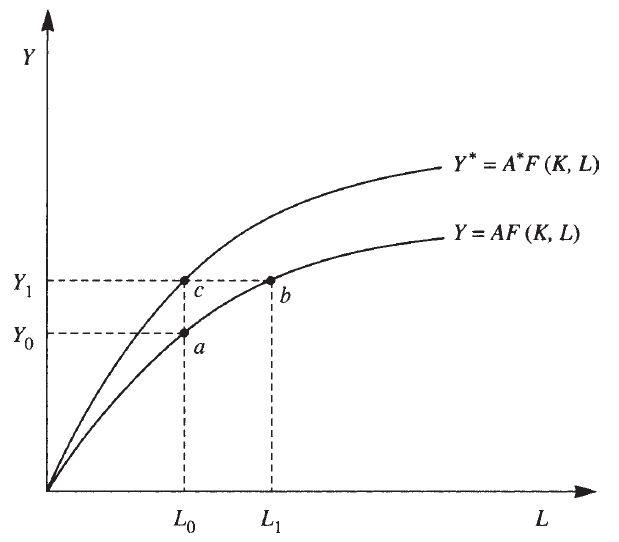
\includegraphics[width=0.5\textwidth]{./figures/aula02_funcaodeproducao.JPG}
        \caption{Função de produção agregada. Fonte: Snowdon e Vane (2005).}
        \label{funcao_producao}
    \end{figure}
\end{frame}

\begin{frame}{Função de produção agregada: propriedades}
    \begin{enumerate}
        \item Dados $A$ e $K$, existe uma \textcolor{purple}{relação positiva entre emprego ($L$) e produto agregado ($Y$)} - movimento ao longo da curva do ponto $a$ para o ponto $b$.\bigskip

        \item A função de produção exibe \textcolor{purple}{rendimentos marginais decrescentes} com relação ao trabalho.\bigskip

              \begin{itemize}
                  \item Aumentos marginais na quantidade de trabalho empregada leva a incrementos cada vez menores no produto.\medskip

                  \item Dado que $\Delta Y/\Delta L$ mede o \textbf{produto marginal do trabalho} (MPL), a inclinação da função de produção nos mostra que um aumento no emprego está associado a um produto marginal do trabalho decrescente. \medskip

                  \item O produto marginal decrescente do trabalho é ilustrado na figura a seguir - $D_L$ é positiva e decrescente.\medskip
              \end{itemize}

        \item A função de produção desloca-se para cima com aumento do estoque de capital e/ou melhorias tecnológicas - Figuras \ref{funcao_producao} e \ref{pml}.
    \end{enumerate}
\end{frame}

\begin{frame}{Função de produção agregada: propriedades}
    \begin{figure}
        \centering
        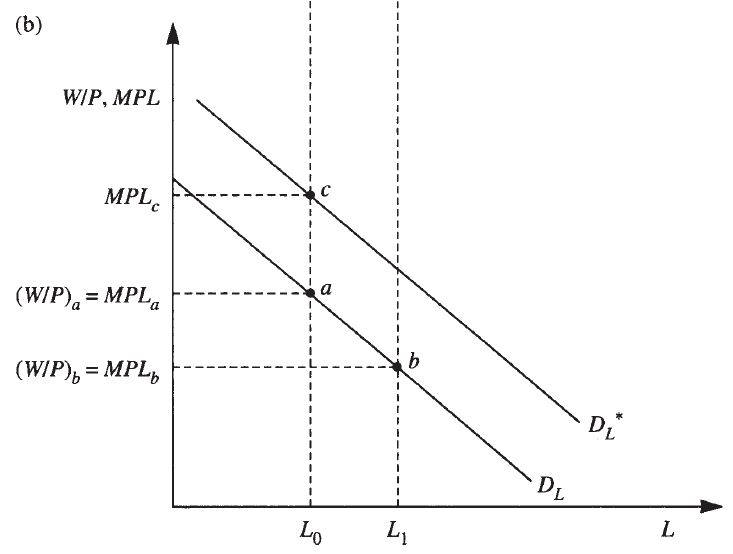
\includegraphics[width=0.6\textwidth]{./figures/aula02_pml.JPG}
        \caption{Produto marginal do trabalho. Fonte: Snowdon e Vane (2005).}
        \label{pml}
    \end{figure}
\end{frame}

\subsection{Emprego}
\begin{frame}{Mercado de trabalho clássico}
    \begin{itemize}
        \item A equação (\ref{eq1}) nos traz bastante informação acerca do relacionamento entre o produto de uma economia e os insumos utilizados.\bigskip

        \item No entanto, não nos diz nada sobre quanto de mão de obra será empregada em um particular período do tempo.\bigskip

        \item Para ver como o nível agregado de emprego é determinado no modelo clássico, precisamos examinar o modelo clássico do mercado de trabalho.
    \end{itemize}
\end{frame}

\begin{frame}{Mercado de trabalho clássico}
    \begin{itemize}
        \item A \tikz[tstyle]{\node[nstyle](node0){análise clássica do mercado de trabalho}} tem como principal hipótese o bom funcionamento dos mercados.\bigskip
              \begin{tikzpicture}[tpstyle]
                  \draw[pencil,brick,very thick] ([yshift=-1pt]node0.south west) to ([yshift=-1pt]node0.south east);
              \end{tikzpicture}

        \item Firmas e trabalhadores individuais são agentes otimizadores.\bigskip

        \item Eles possuem informação perfeita acerca dos preços relevantes.\bigskip

        \item Não existem barreiras de ajustamento dos salários nominais.\bigskip

        \item Os mercados sempre se equilibram.
    \end{itemize}
\end{frame}

\begin{frame}{Demanda por trabalho}
    \begin{itemize}
        \item O quanto de trabalho uma firma maximizadora de lucros demandará?\bigskip

        \item A condição bem estabelecida para maximização de lucros é de que uma firma deve igualar sua receita marginal ($MR_i$) ao custo marginal de produção ($MC_i$).\bigskip

        \item Para uma \textcolor{purple}{firma perfeitamente competitiva}, $MR_i = P_i$, o preço do produto da firma $i$. \bigskip

        \item A condição de maximização de lucros pode ser, então, escrita como:
              \begin{equation}
                  P_i = MC_i.
                  \label{eq2}
              \end{equation}
    \end{itemize}
\end{frame}

\begin{frame}{Demanda por trabalho}
    \begin{itemize}
        \item Se uma firma contrata em um mercado de trabalho competitivo, um salário nominal igual à $W_i$ deve ser pago para cada trabalhador adicional.\bigskip

        \item O custo adicional de contratação de uma unidade extra de trabalho será igual à $W_i\Delta L_i$.\bigskip

        \item A receita adicional gerada por uma unidade extra de trabalho é o produto adicional produzido ($\Delta Q_i$) multiplicado pelo preço do bem produzido por esta firma ($P_i$).\bigskip

        \item A receita adicional é, portanto, igual à $P_i\Delta Q_i$.\bigskip

        \item Uma firma maximizadora de lucros, portanto, contratará mão de obra desde que $W_i\Delta L_i < P_i\Delta Q_i$.
    \end{itemize}
\end{frame}

\begin{frame}{Demanda por trabalho}
    \begin{itemize}
        \item Para maximizar lucros, a seguinte condição deve ser satisfeita:\medskip
              \begin{equation}
                  P_i\Delta Q_i = W_i \Delta L_i.
                  \label{eq3}
              \end{equation}\bigskip

        \item A condição anterior é equivalente a:\medskip
              \begin{equation}
                  \tikz[tstyle]{\node[nstyle](node0){$\frac{\Delta Q_i}{\Delta L_i}$}} = \tikz[tstyle]{\node[nstyle](node1){$\frac{W_i}{P_i}$}}.
                  \label{eq4}
              \end{equation}\bigskip
              \begin{tikzpicture}[tpstyle]
                  \draw[snake,->,brick] ([yshift=2pt]node0.south west) to[bend right] +(-0.7,-0.5) node[anchor=east,opacity=1] {\hand Produto marginal do trabalho};
                  \draw[snake,->] ([yshift=2pt]node1.north east) to[bend left] +(0.7,0.5) node[anchor=west,opacity=1] {\hand Salário real};
              \end{tikzpicture}

        \item A condição (\ref{eq4}) é uma maneira alternativa de expressar a equação (\ref{eq2}) - $P_i = MC_i$.
    \end{itemize}
\end{frame}

\begin{frame}{Demanda por trabalho}
    \begin{itemize}
        \item Dado que $MC_i$ é o custo de um trabalhador adicional ($W_i$) dividido pelo produto adicional produzido por esse trabalhador ($MPL_i$), podemos escrever essa relação como:
              \begin{equation}
                  MC_i = \frac{W_i}{MPL_i}.
                  \label{eq5}
              \end{equation}

        \item Combinando as equações (\ref{eq5}) e (\ref{eq2}), obtemos:
              \begin{equation}
                  P_i = \frac{W_i}{MPL_i} = MC_i.
                  \label{eq6}
              \end{equation}

        \item Como a produtividade marginal do trabalho ($MPL$) é uma função decrescente da quantidade de trabalho empregada - devido aos rendimentos decrescentes - a curva MPL tem inclinação negativa (Figura \ref{pml}).
    \end{itemize}
\end{frame}

\begin{frame}{Demanda por trabalho}
    \begin{itemize}
        \item Lucros são maximizados quando uma firma equaliza $MPL_i$ com $W_i/P_i$, a curva de produto marginal do trabalho é equivalente à curva de demanda por trabalho da firma $i$ ($D_{Li}$).\bigskip

        \item A \tikz[tstyle]{\node[nstyle](node0){curva de demanda por trabalho}} da firma $i$ é expressa pela seguinte relação:
              \begin{equation}
                  D_{Li} = D_{Li}\left(\frac{W_i}{P_i}\right), \qquad D'(\bullet) < 0.
                  \label{eq7}
              \end{equation}\bigskip
              \begin{tikzpicture}[tpstyle]
                  \node[pencil,draw,minimum height=0.7cm,minimum width=5cm] (box0) at (node0) {};
              \end{tikzpicture}

        \item \textcolor{purple}{A demanda por trabalho de uma firma é uma função inversa do salário real}.\bigskip

        \item Quanto menor o salário real, maior a quantidade de mão de obra que será empregada de maneira lucrativa.
    \end{itemize}
\end{frame}

\begin{frame}{Demanda agregada por trabalho}
    \begin{itemize}
        \item A análise feita anteriormente considera o comportamento de uma firma individual.\bigskip

        \item Como a demanda de trabalho de uma firma individual é uma função inversa do salário real, ao agregar essas funções para todas as firmas, obtemos o postulado clássico de que \textcolor{purple}{a demanda agregada de trabalho é uma função inversa do salário real}.\bigskip

        \item A \hlight{fun\c{c}\~{a}o de demanda agregada por trabalho} é expressa por:
              \begin{equation}
                  D_L = D_L\left(\frac{W}{P}\right), \qquad D'_L(\bullet)<0.
              \end{equation}
    \end{itemize}
\end{frame}

\begin{frame}{Oferta agregada de trabalho}
    \begin{itemize}
        \item Agora consideraremos o lado da oferta do mercado de trabalho.\bigskip

        \item Assume-se, no modelo clássico, que as famílias são maximizadoras de utilidade.\bigskip

        \item A oferta de mercado de trabalho é, portanto, uma função positiva do salário real, e é dada pela seguinte expressão:\medskip
              \begin{equation}
                  S_L = S_L\left(\frac{W}{P}\right), \qquad S'_L(\bullet)>0.
                  \label{eq9}
              \end{equation}
    \end{itemize}
\end{frame}

\begin{frame}{Oferta agregada de trabalho}
    \begin{itemize}
        \item A quantidade de trabalho ofertada depende das preferências das famílias com relação a consumo e lazer (ambos trazem utilidade aos agentes).\bigskip

        \item Para consumir, as famílias devem adquirir renda substituindo tempo de lazer por horas de trabalho.\bigskip

        \item No entanto, assume-se que o trabalho traz desutilidade para as famílias.\bigskip

        \item Portanto, as preferências das famílias e o salário real determinarão a quantidade de equilíbrio na oferta de trabalho.
    \end{itemize}
\end{frame}

\begin{frame}{Oferta agregada de trabalho}
    \begin{itemize}
        \item Um aumento no salário real torna o lazer mais caro em termos de ``renda perdida'' e, portanto, tende a aumentar a oferta de \tikz[tstyle]{\node[nstyle](node0){trabalho}}.\bigskip

        \item Por outro lado, um salário real mais alto representa uma melhora na qualidade de vida das famílias e, portanto, eles podem adquirir mais tempo de lazer (reduzindo a oferta de \tikz[tstyle]{\node[nstyle](node1){trabalho}}).\bigskip\bigskip
              \begin{tikzpicture}[tpstyle]
                  \draw[snake,->,note] ([yshift=2pt]node0.south east) to [bend right] +(0.7,-0.3) node[anchor=west] {\hand Efeito substituição};
                  \draw[snake,->,brick] ([yshift=2pt]node1.south east) to [bend left] +(-1.7,-0.3) node[anchor=east] {\hand Efeito renda};
              \end{tikzpicture}
        \item O modelo clássico assume que \textcolor{purple}{o efeito substituição domina o efeito renda, de forma que a oferta de trabalho responde positivamente a aumentos no salário real}.\bigskip
        \item Agora que vimos a derivação das curvas de oferta e demanda por trabalho, estamos em posição para determinar a renda e emprego de equilíbrio competitivo no modelo clássico.
    \end{itemize}
\end{frame}

\subsection{Determinação da renda e do emprego}
\begin{frame}{Determinação da renda e do emprego de equilíbrio}
    \begin{figure}
        \centering
        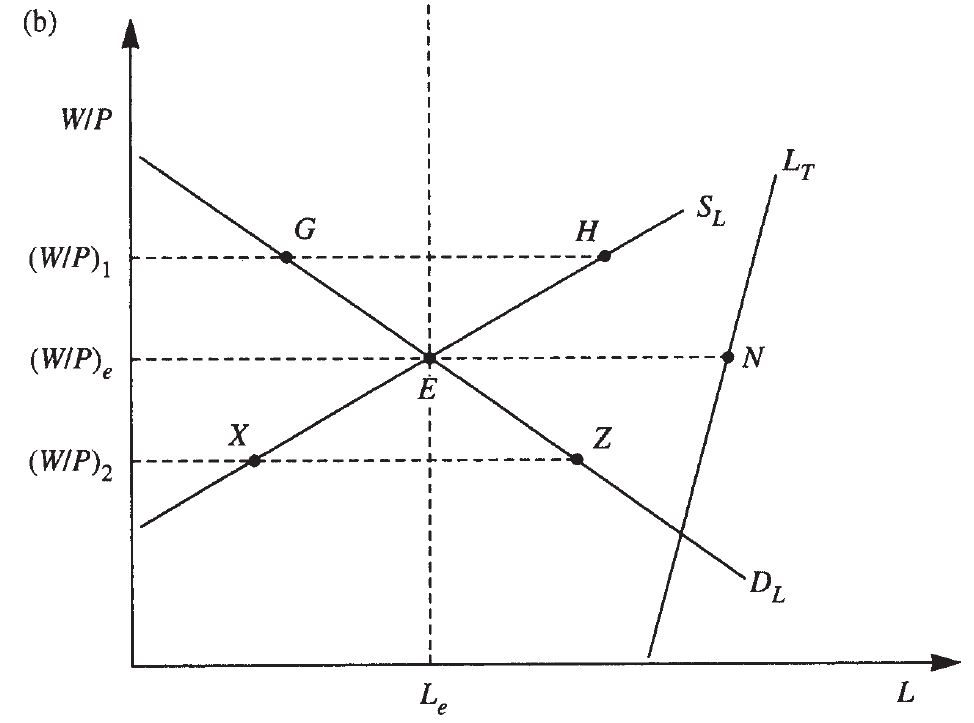
\includegraphics[width=0.6\textwidth]{./figures/aula02_labormarket.JPG}
        \caption{Equilíbrio no mercado de trabalho. Fonte: Snowdon e Vane (2005).}
        \label{fig3}
    \end{figure}
\end{frame}

\begin{frame}{Determinação da renda e do emprego de equilíbrio}
    \begin{itemize}
        \item As forças de demanda e oferta estabelecem um salário real de equilíbrio $(W/P)_e$ e um nível de equilíbrio de emprego $(L_e)$.\bigskip

        \item Se o salário real estiver abaixo do nível de equilíbrio, haveria um excesso de demanda por trabalho na magnitude $ZX$ e, portanto, os salários aumentariam em resposta às propostas salariais das firmas, restaurando o salário real ao seu nível de equilíbrio competitivo.\bigskip

        \item Por outro lado, se o salário real estivesse acima do valor de equilíbrio, haveria um excesso de oferta de trabalho de magnitude $HG$. Neste caso, os salários reais abaixariam até o nível competitivo $(W/P)_e$.\bigskip

        \item Este resultado é garantido no modelo clássico devido às hipóteses de \textcolor{purple}{mercado perfeitamente competitivos, pre\c{c}os flex\'{i}veis e informa\c{c}\~{a}o completa}.
    \end{itemize}
\end{frame}

\begin{frame}{Determinação da renda e do emprego de equilíbrio}
    \begin{itemize}
        \item O nível de emprego em equilíbrio $(L_e)$ representa o \hlight{pleno emprego} nesta economia - todos os membros da força de trabalho que desejam trabalhar pelo dado nível de equilíbrio do salário real conseguiriam.\bigskip

        \item Enquanto a curva $S_L$ indica quantas pessoas estão dispostas a aceitar ofertas de emprego pra cada nível de salário real, a curva $L_T$ indica o número total de pessoas que desejam compor a força de trabalho para cada nível de salário real.\bigskip

        \item A curva $L_T$ é positivamente inclinada, indicando que para níveis mais altos de salários reais, mais pessoas estão dispostas a entrar na força de trabalho.
    \end{itemize}
\end{frame}

\begin{frame}{Determinação da renda e do emprego de equilíbrio}
    \begin{itemize}
        \item No modelo clássico, \textbf{o equilíbrio no mercado de trabalho está associado com um desemprego de magnitude $EN$}.\bigskip

        \item O equilíbrio de pleno emprego clássico é perfeitamente compatível com a existência de desemprego \tikz[tstyle]{\node[nstyle](node0){friccional}} e/ou \tikz[tstyle]{\node[nstyle](node1){voluntário}}.\bigskip

        \item No entanto, \hlight{n\~{a}o admite a possibilidade de exist\^{e}ncia de desemprego involunt\'{a}rio}.\bigskip

        \item Friedman (1968), posteriormente, introduziu o conceito de \tikz[tstyle]{\node[nstyle](node2){taxa natural de desemprego}} ao discutir o desemprego de equilíbrio no mercado de trabalho - veremos mais tarde na disciplina.\bigskip
        \item Uma vez determinado o nível de emprego de equilíbrio no mercado de trabalho, o nível de produto é determinado pela posição da função de produção agregada.
              \begin{tikzpicture}[tpstyle]
                  \node[pencil,draw,minimum height=0.5cm, minimum width=1.6cm,green] (box0) at (node0) {};
                  \node[pencil,draw,minimum height=0.5cm, minimum width=1.7cm,green] (box1) at (node1) {};
                  \draw[pencil,very thick, brick] ([yshift=-1pt]node2.south west) to ([yshift=-1pt]node2.south east);
              \end{tikzpicture}
    \end{itemize}
\end{frame}

\begin{frame}{Determinação da renda e do emprego de equilíbrio}
    \begin{figure}
        \centering
        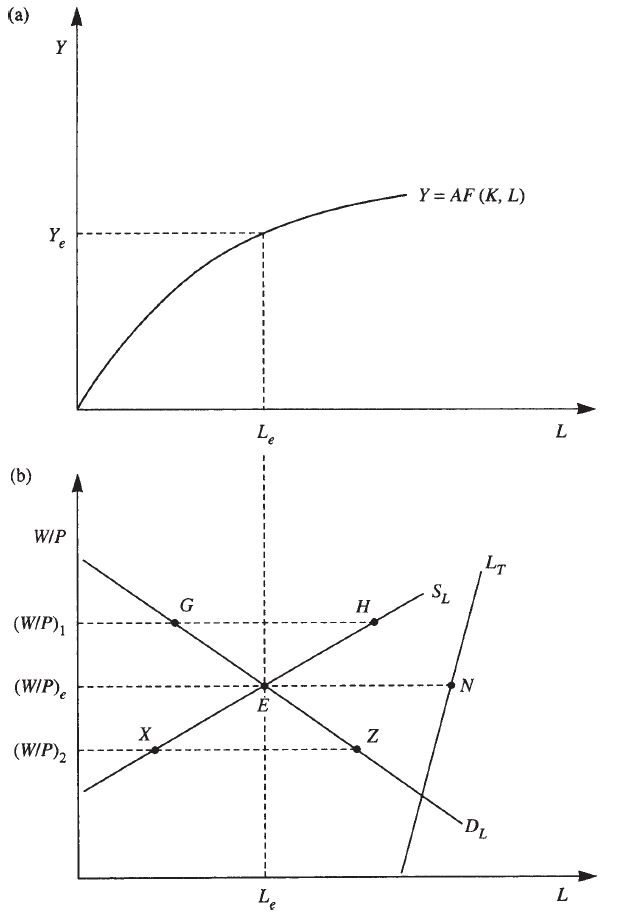
\includegraphics[width=0.3\textwidth]{./figures/aula02_labor.JPG}
        \caption{Determinação da renda e emprego de equilíbrio. Fonte: Snowdon e Vane (2005).}
        \label{fig4}
    \end{figure}
\end{frame}

\section{Conclusões}
\begin{frame}{Conclusões}
    \begin{itemize}
        \item A competição perfeita no mercado de trabalho assegura o pleno emprego no modelo clássico.\medskip

        \item Ao salário real de equilíbrio, nenhuma pessoa que deseja trabalhar a esse nível de salário real está desempregada.\medskip

        \item ``Os postulados clássicos não admitem a possibilidade de desemprego involuntário'' (Keynes, 1936).\medskip

        \item Economistas clássicos tinham ciência que desemprego persistente em excesso com relação ao nível de equilíbrio era possível se impostas restrições artificiais sobre as funções equilibradoras do salário real.\medskip

        \item Se os salários reais fossem mantidos acima do nível de equilíbrio (sindicatos e/ou legislações de salário mínimo), então, nem todos que desejam trabalhar a esse nível `artificial' de salário real conseguiria emprego.\medskip

        \item A solução para o `desemprego clássico' é simples e óbvia - os salários reais devem ser reduzidos diminuindo salários nominais.
    \end{itemize}
\end{frame}

\begin{frame}{Conclusões}
    \begin{itemize}
        \item Keynes argumenta que o nível de equilíbrio verificado na Figura \ref{fig4} é um `caso especial' que não é típico da `sociedade econômica na qual nós vivemos' (Keynes, 1936).\bigskip

        \item O equilíbrio de pleno emprego do modelo clássico é um caso especial pois corresponde a uma situação na qual a demanda agregada é exatamente suficiente para absorver o nível de produto produzido.\bigskip

        \item A objeção de Keynes é de que não existe nada que assegure que a demanda agregada esteja neste nível específico.\bigskip

        \item Os economistas clássicos negavam a possibilidade de deficiência de demanda agregada recorrendo à Lei de Say, que é ``equivalente à proposição de que não existem obstáculos ao pleno emprego'' (Keynes, 1936).\bigskip

        \item Essa proposição será nosso objeto de estudo na próxima aula.
    \end{itemize}
\end{frame}

\section{Bibliografia}
\begin{frame}{Bibliografia \emoji{books}}
    \begin{itemize}
        \item FROYEN, R. \emph{Macroeconomia: teorias e aplicações}. 2.ed. São Paulo: Saraiva, 2013. Disponível em: \href{https://app.minhabiblioteca.com.br/books/9788502175235}{app.minhabiblioteca.com.br/books/9788502175235}\medskip
        \item KEYNES, J.M. \emph{A teoria geral do emprego, do juro e da moeda}. São Paulo: Atlas, 1992. (Data do original em inglês: 1936).\medskip
        \item LOPES, L.M.; VASCONCELLOS, M.A.S. \emph{Manual de Macroeconomia: Nível básico e nível intermediário}. 3.ed. São Paulo: Atlas, 2008.\medskip
        \item SNOWDON, B.; VANE, H.R. \emph{Modern Macroeconomics: its Origins, Development and Current State}. Northampton, MA: Edward Elgar, 2005.
    \end{itemize}
\end{frame}
\end{document}